%PDFLaTeX
%!TEX encoding = UTF-8 Unicode
%!BIB program = bibtex
\documentclass{deumathproject}
% aşağıdaki paketler class dosyasında ekli
%\usepackage{amssymb, amsmath, amsfonts}
%\usepackage{graphicx}
%\usepackage{setspace}
%\usepackage[utf8]{inputenc}

\usepackage{listings}
\usepackage{xcolor}
\usepackage{multicol}

\definecolor{codegreen}{rgb}{0.43,0.57,0.49}
\definecolor{codegray}{rgb}{0.5,0.5,0.5}
\definecolor{codepurple}{rgb}{0.4,0.43,0.58}
\definecolor{codeorange}{rgb}{0.70,0.57,0.51}
%\definecolor{backcolour}{rgb}{0.95,0.95,0.92}
\definecolor{backcolour}{rgb}{0.11,0.12,0.13}
\definecolor{plaincode}{rgb}{0.69,0.72,0.75}

\lstdefinestyle{mystyle}{
    backgroundcolor=\color{backcolour},
    commentstyle=\color{codegreen},
    keywordstyle=\color{codeorange},
    numberstyle=\tiny\color{codegray},
    stringstyle=\color{codepurple},
    basicstyle=\ttfamily\footnotesize\color{plaincode},
    breakatwhitespace=false,
    breaklines=true,
    captionpos=b,
    keepspaces=true,
    numbers=left,
    numbersep=5pt,
    showspaces=false,
    showstringspaces=false,
    showtabs=false,
    tabsize=2
}

\lstset{style=mystyle}


\author{Bahar ÇAKIRGÖZ, Mert GÜÇSAV}
\date{Spring, 2024} %Fall/Spring, 2024 projenin dönemi, yıl, birini sil!
\title{Tangential Cutter\\ with Python} % Büyük harfle
\supervisor{Prof. Dr. Başak KARPUZ}
% Assist. Prof. Dr. <= Dr. Öğr. Üyesi
% Assoc. Prof. Dr. <= Doç. Dr.
% Prof. Dr.  <= Prof. Dr.

%%%%   derse göre birini seçin
%\reportkind{MAT 4079 GRADUATION PROJECT REPORT}
\reportkind{MAT 4070 PROJECT REPORT}
%%%%

\usepackage{amsthm}
\newtheorem{theorem}{Theorem}[chapter]
\newtheorem{corollary}[theorem]{Corollary}
\newtheorem{lemma}[theorem]{Lemma}
\newtheorem{property}[theorem]{Property}
\newtheorem{definition}{Definition}[chapter]
\newtheorem{example}{Example}
% gerekirse başka theorem environment i eklersiniz...


\begin{document}
	\maketitle
	
	\begin{abstract} % özet
	In this project,
    we transform a 3D Printer into a Tangential Cutter in the hardware-wise
    so that it will be able to cut custom stickers.
    On the other hand, in the software-wise, we read some graphics from external files with the programming language Python,
    and translate the graphics into the 3D Printer's language.
	\end{abstract}
	
	\tableofcontents
	\listoffigures  % projede şekil YOK ise bu satırın başına % koy
	%\listoftables   % projede tablo YOK ise bu satırın başına % koy
	
	% Eğer kısaltmalar tablon var ise
	%\startlistofabbreviations
	%\input{kısalmaları barındıran tex dosyasının adı}
	
	% Eğer sembol listen var ise
	%\startlistofsymbols
	%\input{sembol listesini barındıran tex dosyasının adı}	
	
	\clearpage                     %
	\pagenumbering{arabic}         %  bu iki satırı SİLME !!!
	
	\chapter{FDM 3D PRINTERS}

\section{General Information}

Fused Deposition Modeling (FDM) is one of the most popular and widely used 3D printing technologies. Here's some general information about FDM printers:

\noindent\textbf{Principle.}
FDM printers work by heating and extruding thermoplastic filament through a heated nozzle, which deposits layers of material to build up the final object. The filament is fed from a spool into the extruder, where it is melted and extruded onto the build platform layer by layer.

\noindent\textbf{Materials.}
FDM printers can work with a wide range of thermoplastic materials, including PLA (Polylactic Acid), ABS (Acrylonitrile Butadiene Styrene), PETG (Polyethylene Terephthalate Glycol), TPU (Thermoplastic Polyurethane), and many others. Each material has its own properties in terms of strength, flexibility, temperature resistance, and surface finish.

\noindent\textbf{Build Volume.}
FDM printers are available in various sizes and configurations, with different build volumes to accommodate different project requirements. Desktop FDM printers are commonly used for prototyping, hobbyist projects, and small-scale production, while larger industrial FDM printers are used for manufacturing and production applications.

\noindent\textbf{Layer Resolution.}
FDM printers can achieve varying levels of layer resolution, ranging from coarse to fine, depending on factors such as nozzle size, layer height, and print speed. Smaller layer heights result in finer details and smoother surface finishes but may require longer print times.

\noindent\textbf{Support Structures.}
FDM printers often require support structures to be added to overhanging or bridging areas of the print to prevent sagging or collapsing during printing. These supports are typically made from the same material as the print and are removed after printing is complete.

\noindent\textbf{Post-Processing.}
After printing, FDM parts may require post-processing to improve their surface finish or mechanical properties. This can include sanding, painting, smoothing with solvents or heat, or annealing (for certain materials like ABS).

\noindent\textbf{Applications.}
FDM printers are used in a wide range of industries and applications, including prototyping, product design, manufacturing, education, healthcare, aerospace, automotive, and consumer goods. They are valued for their affordability, versatility, and ease of use.

\noindent\textbf{Open-Source Community.}
FDM printing has a vibrant open-source community that has contributed to the development of hardware, software, and materials. This community-driven approach has led to innovations in printer design, materials development, and software tools, making FDM printing more accessible and affordable for enthusiasts and professionals alike.
Overall, FDM printing is a versatile and accessible 3D printing technology that continues to evolve and expand its capabilities for a wide range of applications.


\section{Kinematic System Types}

These are just a few examples of the many kinematic systems used in 3D printers.
Each system has its own advantages, limitations, and applications, and the choice of kinematic system depends on factors such as printing speed, accuracy, build volume, and intended use.

\noindent\textbf{Cartesian.}
Cartesian 3D printers use a rectangular coordinate system with three linear axes  $(x,y,z,e)$ to move the print head and build platform.
This is the most common type of kinematic system used in desktop 3D printers.

\noindent\textbf{Delta.}
Delta printers use three vertical columns with parallel arms connected to the print head. By varying the length of the arms, the printer can precisely control the movement of the print head in three dimensions.
Delta printers are known for their fast printing speeds and are often used for tall and cylindrical prints.

\noindent\textbf{CoreXY.}
CoreXY printers use two stationary stepper motors to drive belts that move the print head along the $x$ and $y$ axes.
This configuration allows for simultaneous movement in both directions without the need for heavy motors on the moving carriage, resulting in smoother and faster motion.

\noindent\textbf{H-Bot.}
H-Bot printers use two parallel rails or tracks with a carriage that moves along each track.
The carriages are connected by a crossbeam, forming the {\textquotedblleft}H{\textquotedblright} shape.
H-Bot mechanisms allow for compact and lightweight designs, making them suitable for desktop and small-scale 3D printers.

\noindent\textbf{Scara.}
SCARA (Selective Compliance Assembly Robot Arm) printers use a robotic arm
with two parallel joints (shoulder and elbow) to control the movement of the print head.
SCARA printers are known for their speed and accuracy and are often used in industrial applications.


\noindent\textbf{Pola.}
Polar printers use a rotating build platform and a print head that moves along radial and angular axes. This configuration allows for printing objects with a cylindrical or spherical shape and is often used for specialized applications such as printing round objects or sculptures.


\section{Artillery Sidewinder X2}

The Artillery Sidewinder X2 is a 3D printer produced by Artillery, a manufacturer known for its reliable and affordable printers. The Sidewinder X2 is an upgraded version of the original Sidewinder, boasting several improvements and enhancements.

Some key features of the Artillery Sidewinder X2 include:

\noindent\textbf{Large Build Volume.}
It offers a spacious build volume, allowing users to create relatively large 3D prints compared to many other printers in its price range.

\noindent\textbf{Dual $Z$-Axis.}
The Sidewinder X2 features a dual $Z$-axis design, which helps in ensuring more stable and precise vertical movement during printing, resulting in improved print quality.

\noindent\textbf{Direct Drive Extruder.}
It utilizes a direct drive extruder system, which is known for better filament control and compatibility with a wider range of filament types,
including flexible materials.

\noindent\textbf{Touchscreen Interface.}
The printer is equipped with a touchscreen interface, making it easy to navigate and control various settings and functions.

\noindent\textbf{Fast Printing Speed.}
It is capable of printing at relatively high speeds while maintaining print quality,
thanks to its robust construction and efficient design.

\noindent\textbf{Silent Printing.}
The Sidewinder X2 is known for its relatively quiet operation,
which is achieved through the use of high-quality stepper motors and other noise-reducing components.

Overall, the Artillery Sidewinder X2 is popular among 3D printing enthusiasts and hobbyists for its combination of large build volume,
reliable performance, and affordable price point.

\begin{figure}[h!tb]
\centering
\begin{multicols}{3}
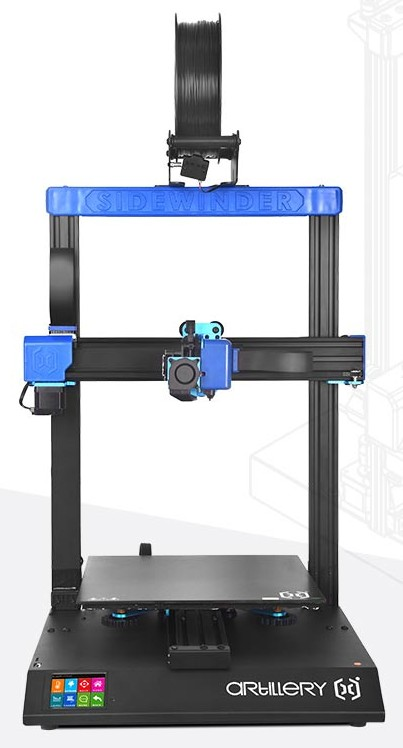
\includegraphics[scale=0.20]{x2-f1-edited.jpg}\par
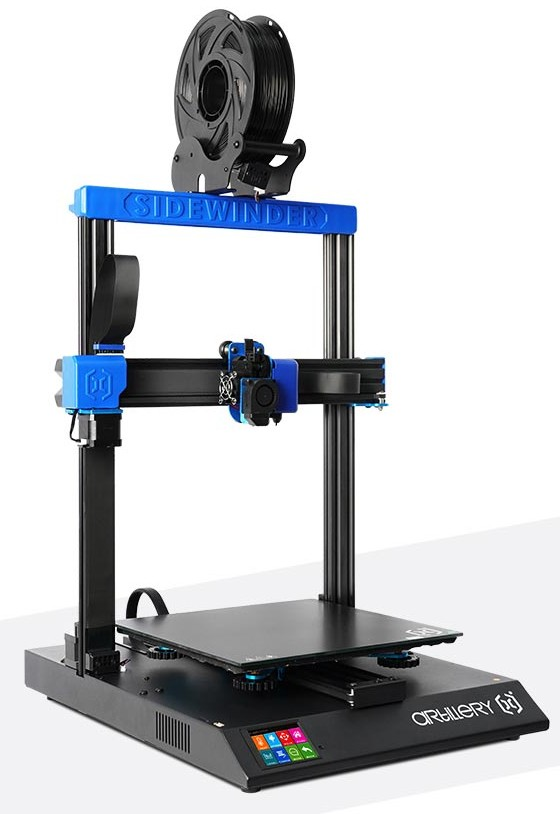
\includegraphics[scale=0.20]{x2-f2-edited.jpg}\par
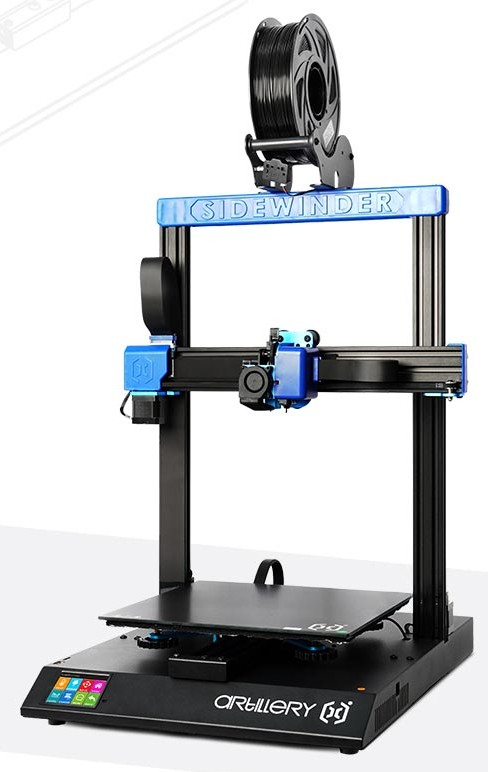
\includegraphics[scale=0.20]{x2-f3-edited.jpg}
\end{multicols}
%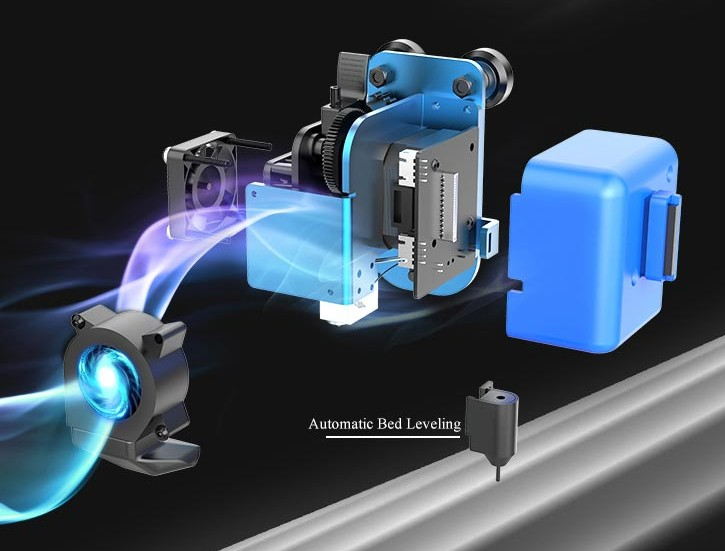
\includegraphics[scale=0.15]{x2-e-edited.jpg}
\caption{Artillery Sidewinder X2}
\label{fig:label1}
\end{figure}

\begin{figure}[h!tb]
\centering
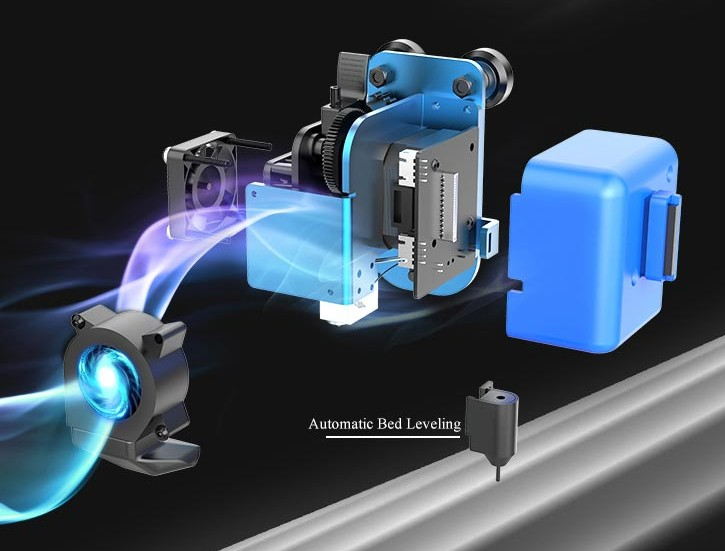
\includegraphics[scale=0.40]{x2-e-edited.jpg}
\caption{Artillery Sidewinder X2 - Extruder}
\label{fig:label2}
\end{figure}


%\noindent örnek tablo.
%
%\begin{table}[h]
%	\centering
%		\begin{tabular}{cccc}
%			\hline\hline
%			$ N $   & $ n=3 $ & $ n=4 $ & $ n=5 $ \\
%			\hline
%			20/40   & 1.69    & 2.86    & 3.88    \\
%			40/80   & 1.88    & 2.94    & 3.94    \\
%			80/160  & 1.95    & 2.97    & 3.99    \\
%			\hline\hline
%		\end{tabular}
%	\caption{Bla bla bla...}\label{tab:label}
%\end{table}
%
%\section{Section başlığı 2}
%\subsection{SubSection örneği}
%Citetion örneği: \cite{allaire2008numerical}.

 % birinci CHAPTER içinde barındıran tex dosyası
	\chapter{TANGENTIAL CUTTER}


\section{General Information}

A tangential cutter is a type of cutting tool commonly used in CNC machining
for cutting materials such as vinyl, fabric, foam, and other thin or flexible materials.
Unlike traditional rotary cutters that rotate about a central axis,
tangential cutters have a cutting edge that moves tangentially to the material being cut.

\begin{figure}[h!tb]
\centering
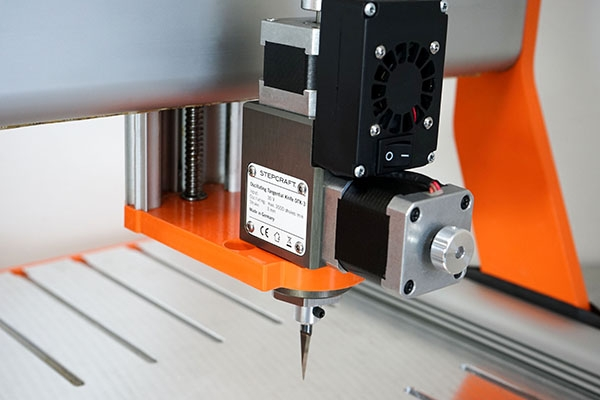
\includegraphics[scale=0.80]{otc.jpg}
\caption{A Tangential Cutter}
\label{fig:label3}
\end{figure}


Here's some information about tangential cutters.

\noindent\textbf{Principle of Operation.}
Tangential cutters work by moving the cutting edge along a linear path, perpendicular to the material surface, while maintaining a fixed orientation relative to the material.
This allows for precise and controlled cutting of intricate shapes and patterns, particularly in thin or flexible materials that may be prone to tearing or distortion with traditional rotary cutters.

\noindent\textbf{Design.}
Tangential cutters typically consist of a blade or cutting tip mounted on a mechanism that allows for precise control of the cutting angle and depth.
The cutting edge may be a straight blade, a beveled blade, or a specialized cutting tip depending on the application and material being cut.
The cutter is attached to a CNC machine's tool holder and is controlled by the machine's software to follow the desired cutting path.

\noindent\textbf{Applications.}
Tangential cutters are commonly used in applications such as sign making, textile cutting, gasket fabrication, packaging, and prototyping.
They are particularly well-suited for cutting intricate designs, small details, and sharp corners in materials that may be difficult to cut with traditional rotary cutters.

\noindent\textbf{Versatility.}
Tangential cutters can be used with a wide range of materials, including vinyl, fabric, leather, foam, paper, cardboard, and more.
They are capable of cutting both straight lines and complex curves with high precision and repeatability.

\noindent\textbf{Software Control.}
Tangential cutters are typically controlled by CNC software that generates toolpaths based on the desired cutting pattern or design.
The software calculates the optimal path for the cutter to follow, taking into account factors such as cutting speed, depth of cut, and corner handling to achieve the desired cut quality and accuracy.

\noindent\textbf{Advantages.}
Tangential cutters offer several advantages over traditional rotary cutters, including greater precision, reduced material waste, improved cut quality, and the ability to cut thicker or more rigid materials without distortion.
They are also capable of cutting small features and sharp corners with high accuracy.

Overall, tangential cutters are versatile and precise cutting tools commonly used in CNC machining for cutting a wide range of materials with high accuracy and repeatability.
Their ability to cut intricate designs and handle thin or flexible materials makes them valuable tools in various industries and applications.

\section{Transforming a 3D Printer into a Tangential Cutter}

To transform a FDM 3D Printer,
we reposition the extruder stepper motor in such a way that
we can attach a blade on the shaft of the stepper motor and revolve it at given angles.
To this end, we used a mont as given in the following graphic.

%{\Huge !!!Insert Graphic - Blade Mount!!!}

\begin{figure}[h!tb]
\centering
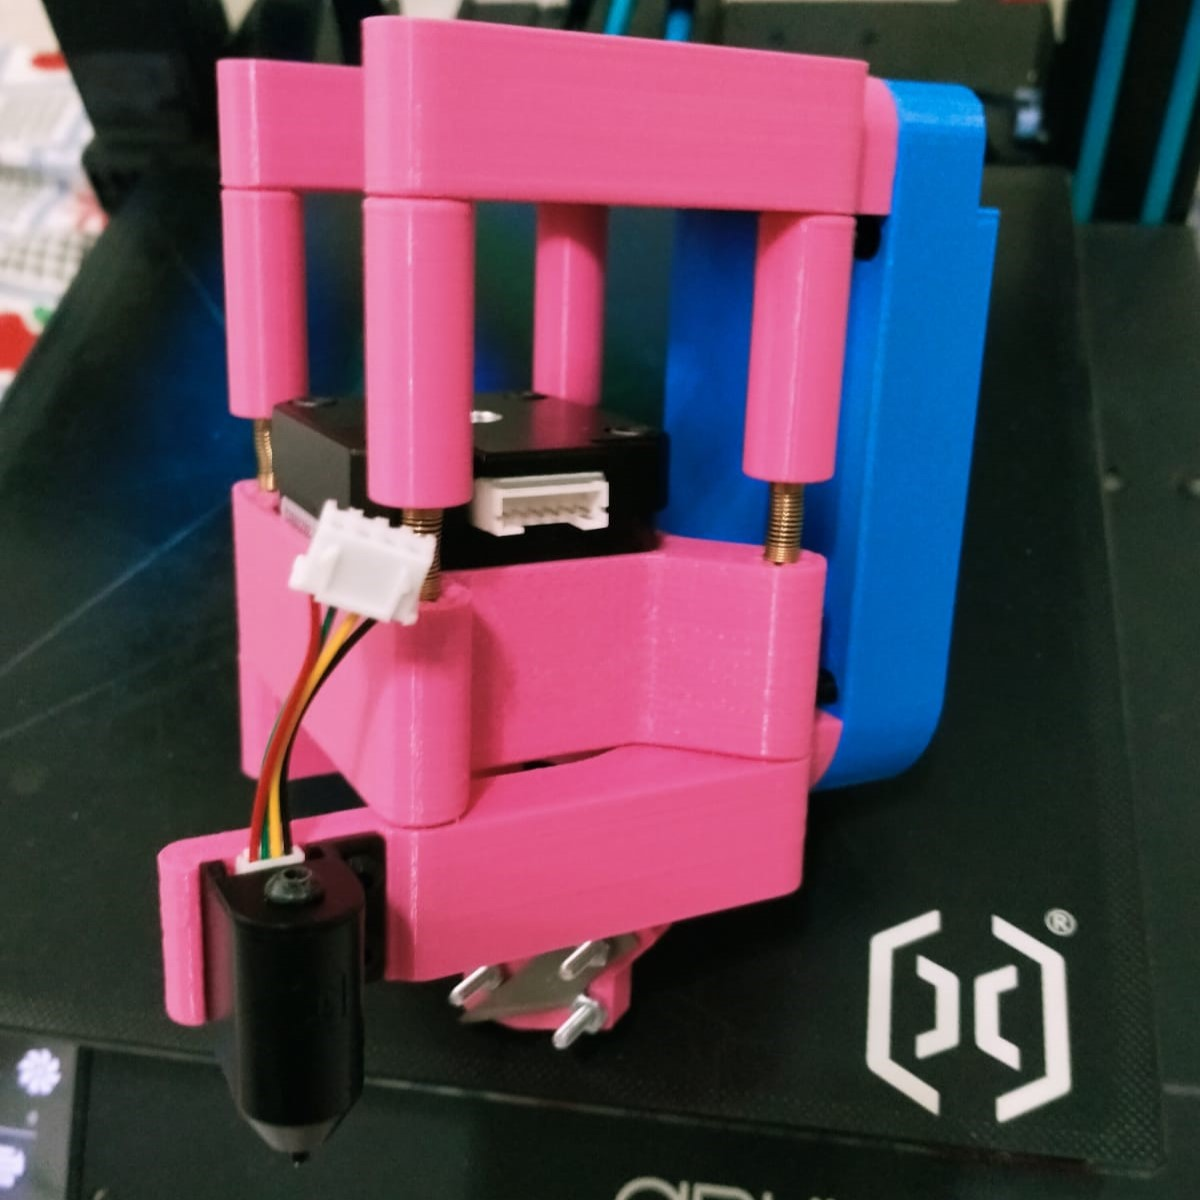
\includegraphics[scale=0.30]{tc-3.jpg}
%\rule{50mm}{50mm}
\caption{Tangential Cutter - Blade Mount}
\label{fig:label4}
\end{figure}


%{\Huge !!!Insert Graphic - Tangential Cutter!!!}

\begin{figure}[h!tb]
\centering
%\rule{50mm}{50mm}
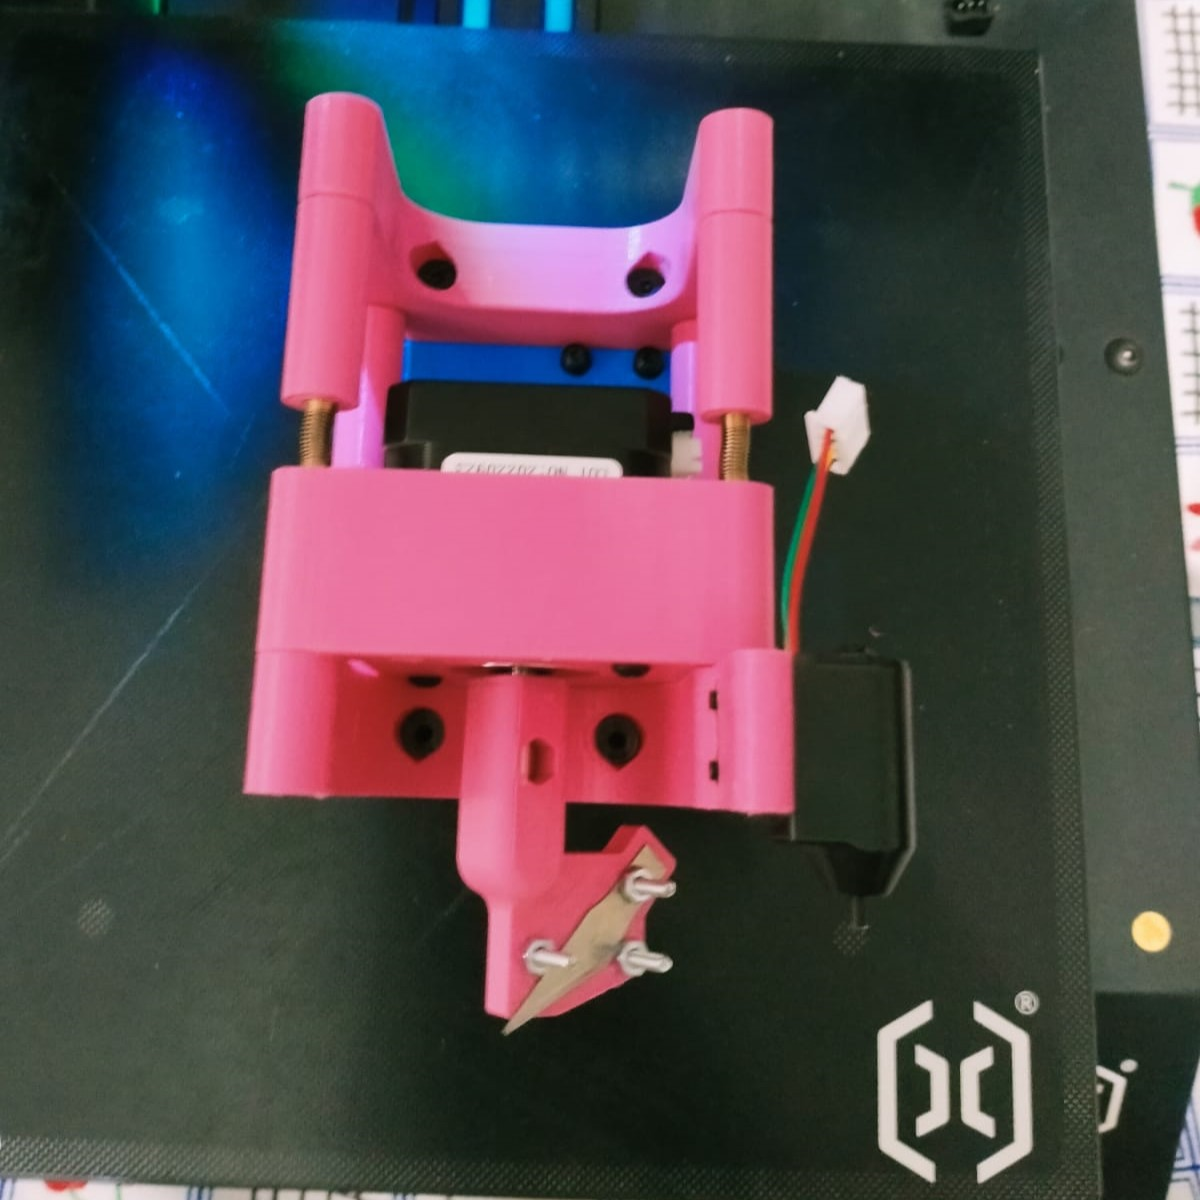
\includegraphics[scale=0.30]{tc-4.jpg}
\caption{Artillery Sidewinder X2 Modified as a Tangential Cutter}
\label{fig:label5}
\end{figure} 
	\chapter{MATHEMATICS}

In this chapter, we explain the figures' mathematical characteristics that we created with the fusion applications DXF files.
\section{Planar Curves}
A planar curve is a curve that, although it may exist in a higher-dimensional space, can be projected or embedded onto a plane without intersections or overlapping parts, effectively making it topologically equivalent to a curve that lies completely within a two-dimensional plane. This property means that even if the curve's original formulation is in three dimensions (or higher), its structure allows it to be represented in two dimensions without loss of essential characteristics, such as connectivity or general shape.
\section{Tangent Lines}
In the realm of mathematical analysis, the tangent line to a curve at a particular point is a critical construct that bridges geometric intuition with analytical rigor. This line touches the curve at a single point and matches the slope of the curve precisely at that point. This connection between a curve and its tangent line can be elucidated using the principles of calculus, specifically through the derivative of the function that describes the curve.

\noindent\textbf{Derivative and the Slope of the Tangent Line.}
The foundation of understanding tangent lines lies in the concept of the derivative. The derivative of a function at any point gives the slope of the tangent line to the function at that particular point. Mathematically, if a function
$y=f(x)$ represents a curve, the derivative
$f^{\prime}(x)$ denotes the slope of the tangent line at any given value of $x$.

\noindent\textbf{Formulating the Equation of a Tangent Line.}
To derive the equation of a tangent line to a curve at a specific point
$x=a$, we employ the following systematic methodology:
\begin{itemize}
\item \textbf{Determine the Derivative.}
    Compute $f^{\prime}(a)$, the derivative of $f$ evaluated at the point $x=a$.
    This value represents the slope of the tangent line at $x=a$.
\item \textbf{Utilize the Point-Slope Form.}
    The point-slope formula, $y-y_{0}=m(x-x_{0})$,
    where $m$ is the slope and $(x_{0},y_{0})$ is a known point on the line, is essential here. For the tangent line,
    we substitute $m=f^{\prime}(a)$ and $(x_{0},y_{0})=(a,f(a))$
\item \textbf{Substitute and Rearrange.}
    Incorporating these values into the point-slope equation provides
    \begin{equation}
    y=f^{\prime}(a)(x-a)+f(a),\nonumber
    \end{equation}
    which upon rearrangement, yields the equation of the tangent line at $x=a$.
\end{itemize}


\section{Some Fundamental Curves}

\subsection{Lines}
A line is a one-dimensional figure, which has length but no width.
Line is made of a set of points which is extended in opposite directions infinitely.
It is determined by two points in a two-dimensional plane.
The two points which lie on the same line are said to be collinear points.

The general equation of straight line is
\begin{equation}
ax+by+c=0\nonumber
\end{equation}
where $a,b,c$ are constants, $x$ and  $y$ are variables and $(-\frac{a}{b})$ is slope.
This equation can also be represented in the parametric form as
\begin{equation}
(t,-\tfrac{a}{b}t-\tfrac{c}{b})\quad\text{for}\ t\in\mathbb{R}.\nonumber
\end{equation}


\subsection{Circles and Circular Arcs}
In geometry, a circle is a special kind of ellipse which the set of all the points in the plane is equidistant from a given point called {\textquotedblleft}centre{\textquotedblright}.
Every line that passes through the circle forms the line of reflection symmetry.
Also, it has rotational symmetry around the centre for every angle.
The circle formula is
\begin{equation}
(x-a)^{2}+(y-b)^{2}=r^{2}\nonumber
\end{equation}
where $(x,y)$ are the coordinate points,
$(a,b)$ is the coordinate of the centre of a circle,
$r$ is the radius of a circle.
The equation of a circle can also be represented in the parametric form as
\begin{equation}
\bigl(r\cos(t)+a,r\sin(t)+b\bigr)\quad\text{for}\ 0\leq{}t<2\pi.\nonumber
\end{equation}
Let $(p,q)$ be a point on a the circle,
then the tangent line of the circle through the points $(p,q)$ is given by
\begin{equation}
\bigl(r\cos(t)+a,r\sin(t)+b\bigr)\quad\text{for}\ 0\leq{}t<2\pi.\nonumber
\end{equation}
where $(p,q)=\bigl(r\cos(\theta_{0})+a,r\sin(\theta_{0})+b\bigr)$ for some $0\leq\theta_{0}<2\pi$.

\subsection{Circular Arcs}
Circular arcs are portions of the circumference of a circle.
In addition to the data for circles, they are defined by two angles:
the starting angle and the ending angle.
Therefore, their parametric formula can be given by
\begin{equation}
\bigl(r\cos(t)+a,r\sin(t)+b\bigr)\quad\text{for}\ \theta_{1}\leq{}t\leq\theta_{2}.\nonumber
\end{equation}


\subsection{Ellipses}
An ellipse is a set of points $(x, y)$ in a Cartesian plane satisfying an equation of the form \begin{equation}
\biggl(\frac{x}{a}\biggr)^{2}+\biggl(\frac{y}{b}\biggr)^{2}=1,\nonumber
\end{equation}
where $a$ is the distance from the origin to the end of
the $x$-axis on the ellipse (semimajor axis),
$b$ is the distance from the origin to the end of
the $y$-axis on the ellipse (semiminor axis), and $a>b$.
The equation of an ellipse can have other forms, but this one,
with the center at the origin and the major axis coinciding with one of the coordinate axes,
is the simplest.
The equation of an ellipse can also be represented in the parametric form as
\begin{equation}
\bigl(a\cos(t),b\sin(t)\bigr)\quad\text{for}\ 0\leq{}t<2\pi.\nonumber
\end{equation}


\subsection{Spline}
Splines are a mathematical and computational tool used extensively for creating smooth and flexible curves through a given set of points, or for function approximation across a domain. In its most basic form, a spline is a piecewise-defined function, typically polynomial in each piece. The overall curve aims to achieve smoothness and minimal curvature, making splines especially valuable in computer graphics, data fitting, and numerical simulation domains.

\subsubsection{B-Spline}

B-Splines, or Basis Splines, offer a robust way to construct these piecewise polynomials,
providing great flexibility and precision.
A B-spline is defined by its order, degree, control points, and a knot vector \cite{allaire2008numerical}.
\begin{itemize}
\item \textbf{Degree (p).} This is the degree of the polynomial in each segment.
    The degree plus one equals the order of the spline.
    For instance, a cubic spline has a degree of three.
\item \textbf{Control Points.} These are the points in a multidimensional space that guide the shape of the spline.
    The spline does not necessarily pass through these points (except in certain conditions like for Bezier curves),
    but they influence the curvature and bending of the spline.
\item \textbf{Knot Vector.} This is a sequence of parameter values that determines where
    and how the control points affect the B-spline curve.
    The knot vector divides the parametric space into intervals
    and influences the continuity and smoothness across the segments of the spline.
\end{itemize}

A B-spline curve is mathematically expressed as:
\begin{equation}
f(t):=\sum_{i=0}^{n}P_{i}B_{i,p}(t),\nonumber
\end{equation}
where
\begin{itemize}
\item $f(t)$ is the point on the B-spline curve at a parameter value $t$.
\item $P_{i}$ are the control points.
\item $B_{i,p}$ are the B-spline basis functions of degree $p$ related to the knot vector.
\end{itemize}
The B-spline basis functions, $B_{i,p}(t)$, are recursively defined by
\begin{equation}
B_{i,0}(t):=
\begin{cases}
1 & \text{if}\ t_{i}\leq{}t < t_{i+1} \\
0 & \text{otherwise}
\end{cases}\nonumber
\end{equation}
and
\begin{equation}
B_{i,p}(t):=\frac{t-t_{i}}{t_{i+p}-t_{i}}B_{i,p-1}(t)+\frac{t_{i+p+1}-t}{t_{i+p+1}-t_{i+1}}B_{i+1,p-1}(t)\quad\text{for}\ n\in\mathbb{N}.\nonumber
\end{equation}
The elegant construction of B-splines using these basis functions allows for local control of the curve
(adjusting one control point only affects the curve locally, within a few segments),
and varying the knot vector can produce different levels of smoothness and curve complexities.
This makes B-splines incredibly powerful and flexible for practical applications like CAD/CAM systems,
animation, and shape modeling. 
	\chapter{DXF FILES(Drawing Exchange Format)}


\noindent\textbf{File Format.} DXF is a file format developed by Autodesk as a universal format
for exchanging CAD data between different software applications.
It is a text-based format, meaning that the file can be opened and viewed with a simple text editor.

\noindent\textbf{Compatibility.} DXF files are widely supported by various CAD (Computer-Aided Design)
and graphics software applications.
They serve as a common interchange format,
allowing users to transfer drawings
and designs between different programs without loss of data or formatting.

\noindent\textbf{Versioning.} DXF has gone through several versions since its inception,
with each version introducing new features and improvements.
Autodesk regularly updates the DXF format to accommodate advancements in CAD technology
and to maintain compatibility with its own software products.

\noindent\textbf{Content.} DXF files can contain various types of drawing elements,
including lines, arcs, circles, polygons, text, and dimensions.
Additionally, they can store layer information, object properties,
and metadata, allowing for rich and detailed drawings.

\noindent\textbf{Use Cases.} DXF files are commonly used for sharing CAD drawings and designs across different platforms
and software applications.
They are widely used in industries such as architecture,
engineering, construction, manufacturing, and graphic design.

\noindent\textbf{Interoperability.} One of the key advantages of DXF files is their interoperability.
Since they are supported by numerous CAD and graphics software programs,
DXF files facilitate collaboration and communication between users
who work with different software tools.

\noindent\textbf{Export and Import.} Most CAD software applications provide options to export drawings to DXF format,
allowing users to share their work with others who may use different software.
Similarly, DXF files can be imported into CAD software for editing, manipulation, and further refinement.

\noindent\textbf{Customization.} DXF is a flexible format that allows for customization and extension.
Users can define their own drawing elements and properties within the DXF file,
making it adaptable to a wide range of design requirements and specifications.
Overall, DXF files play a crucial role in facilitating interoperability
and collaboration in the CAD and design industries,
making them a valuable asset for professionals and enthusiasts alike.

%{\Huge Add References}
\begin{enumerate}
\item Adobe Illustrator
\item AutoCAD
\item Autodesk Fusion 360
\item Blender
\item FreeCAD
\item OpenSCAD
\item Tinkercad
\end{enumerate}


	\chapter{G-CODES: The Language of CNC Machines}


G-Code, short for {\textquotedblleft}Geometric Code{\textquotedblright} or {\textquotedblleft}Gestalt Code{\textquotedblright}, is a language used to control CNC (Computer Numerical Control) machines such as 3D printers, CNC mills, lathes, routers, and laser cutters.
The idea originated in the mid-20th century during the development of the first numerical control (NC) systems for machining.
While the specific individuals responsible for their invention may not be easily identifiable, G-Codes emerged from collaborative efforts among engineers, researchers, and programmers, particularly at institutions like the Massachusetts Institute of Technology (MIT) and within the manufacturing industry during the 1950s and 1960s  (see \cite{marlinfwweb}).
G-Code consists of a series of commands or instructions that tell the machine how to move, position, and operate the cutting tool or print head to create a desired object or part.

Here are some key aspects of G-Codes:

\noindent\textbf{Commands.}
G-Code commands are alphanumeric codes preceded by a letter, such as G, M, T, or S, followed by numerical values or parameters.
Each command corresponds to a specific action or function, such as movement, tool selection, spindle speed, or coolant control.

\noindent\textbf{Coordinate System.}
G-Code uses a coordinate system to specify the position and movement of the machine's axes.
Commonly, this system consists of three linear axes $(x,y,z)$ for 3D printers and CNC mills,
along with additional axes for rotary or angular movement in certain machines.

\noindent\textbf{Motion Control.}
G-Code commands control various aspects of motion, including linear moves, arc moves,
rapid positioning, feed rates (speed of movement), acceleration, and deceleration.
These commands dictate how the machine moves the cutting tool or print head to create the desired shapes and contours.

\noindent\textbf{Tool Control.}
G-Code includes commands for controlling the cutting tool or print head,
such as tool selection, tool change, spindle speed (RPM), direction of rotation, and tool engagement.
These commands determine how the machine operates and interacts with the material being processed.

\noindent\textbf{Program Structure.}
G-Code programs are typically structured as a series of sequential commands organized into blocks or lines of code.
Each line of code represents a specific action or operation to be performed by the machine.
G-Code programs can also include conditional statements, loops, and subroutines for more complex operations.

\noindent\textbf{Post-Processing.}
G-Code files are generated by CAM (Computer-Aided Manufacturing) software based on a 3D model or design.
The CAM software translates the design into a series of G-Code commands tailored to the specific machine and manufacturing process.
These G-Code files can then be loaded into the CNC machine's controller for execution.

Overall, G-Code is a fundamental component of CNC machining and 3D printing,
providing precise control over the manufacturing process
and enabling the creation of complex and intricate parts with high accuracy and repeatability.

\section{Some G-Codes}
In this section, we will review some G-Codes that were used in our project.

\noindent\textbf{G0.}
The G0 command in CNC programming instructs the machine to rapidly move to a specified position
without machining along the way, operating at its maximum traverse speed.
Used primarily for repositioning the tool or machine swiftly between machining locations
or to a starting point for a new operation, G0 commands are essential for efficient CNC machining processes.
However, it's crucial to consider safety, as rapid movements can lead to collisions
or hazards if not carefully controlled within the machining program.

\noindent\textbf{G1.}
The G1 command in CNC programming directs the machine to move in a straight line from its current position to a specified endpoint at a controlled feed rate, allowing for material removal during the motion. This command is fundamental for shaping and machining operations, as it enables precise control over the tool's path and speed, resulting in accurate workpiece fabrication. Unlike the rapid movements of G0, G1 commands involve cutting or material removal, making them essential for achieving the desired dimensions and surface finish of the machined part. As with all CNC commands, proper programming and consideration of safety measures are crucial to ensure efficient and safe machining processes.

\noindent\textbf{G92.}
The G92 command in CNC programming allows for the establishment of a new reference position or coordinate system on the machine. When issued, G92 instructs the machine to set its current position to the specified coordinates, effectively resetting the coordinate system origin. This command is particularly useful for workpiece setup and zero-point definition, enabling operators to designate a specific location as the reference point for subsequent machining operations. By redefining the coordinate system origin, G92 facilitates accurate positioning and machining of parts, streamlining production processes and enhancing overall precision. Proper utilization of the G92 command is essential for ensuring consistency and repeatability in CNC machining tasks, ultimately contributing to the production of high-quality components.

\noindent\textbf{M92.}
The M92 code is typically used in 3D printing rather than CNC machining. In 3D printing, M92 is a command that sets the steps per unit for each axis of the printer. This command allows calibrating the printer to ensure accurate movement according to the specified dimensions in the design files. By adjusting the steps per unit, users can correct any discrepancies between the physical movement of the printer's motors and the intended movements in the 3D model. Proper calibration with the M92 command is crucial for achieving precise and accurate prints, ensuring that the final objects match the intended dimensions and details specified in the design.


%E88.8889; Calibrate E Stepper Motor, E445; Calibrate E Stepper Motor Back

\noindent\textbf{M302.}
The M302 code is used in some 3D printing firmware to enable or disable cold extrusion prevention. In 3D printing, cold extrusion prevention is a safety feature designed to prevent the extruder from operating if the hotend temperature is below a certain threshold. The M302 command allows users to override this safety measure, enabling extrusion even when the hotend is cold. This feature can be useful for troubleshooting or performing maintenance tasks that require manual control over the extrusion process. However, it's important to exercise caution when using M302, as extruding filament at low temperatures can lead to poor print quality, clogs, or other issues. Proper understanding and careful use of the M302 command can help ensure safe and efficient 3D printing operations.

%P1; Disable Cold Extrusion Prevention, P0; Enable Cold Extrusion Prevention


	\chapter{PYTHON}

In this chapter we will be talking about the Pyhton libraries we used in the code (see \cite{pythonweb}).

\section*{EZDXF}

EZDXF is a Python interface to the DXF (drawing interchange file) format developed by Autodesk, ezdxf allows developers to read and modify existing DXF documents or create new DXF documents.

The main objective in the development of EZDXF was to hide complex DXF details from the programmer but still support most capabilities of the DXF format. Nevertheless, a basic understanding of the DXF format is required, also to understand which tasks and goals are possible to accomplish by using the DXF format.

We used EZDXF library to read data from an existing DXF document.

\begin{lstlisting}[language=Python]
import ezdxf
doc=ezdxf.readfile(filename)
\end{lstlisting}

In this code block we access the model space of the DXF file, where all the entities (shapes) are stored.

\begin{lstlisting}[language=Python]
msp=doc.modelspace()
\end{lstlisting}

That way we can read our entities types and with the read types we can carry out operations.

For example:
\begin{lstlisting}[language=Python]
for entity in msp:
if entity.dxftype()=="LINE":
    print_entity(entity)
\end{lstlisting}


\section*{Matplotlib}
 Matplotlib makes it easier to analyze metrics when they are presented in plots,
 which clarify dynamics and trends in seconds, rather than in a huge set of data.
 Matplotlib is a tool that allows your program to speak in a visual way and turn your data into graphs,
 pie charts, bar charts, and more.
 We used this library to visualize the data's inside the DXF files that we read by using the EZDXF library.
 For example:
\begin{lstlisting}[language=Python]
plt.plot(x_bspline_points,y_bspline_points,`b-')
plt.plot(x_bspline_points,y_bspline_points,`bo-',label=`BSpline Points',alpha=0.75)
\end{lstlisting}        
With this example we draw B-Spline points on $xy$ coordinate plane according to their $x$ and $y$ values.
 
\section*{Numpy}

NumPy is a fundamental library in Python, renowned for its support for large,
multi-dimensional arrays and matrices,
along with a comprehensive collection of mathematical functions to operate on these arrays.

This function is able to create an array:
\begin{lstlisting}[language=Python]
create_Array=numpy.array(object,dtype=None,*,copy=True,order=`K',subok=False,ndmin=0,like=None)
\end{lstlisting}   

This function is able to return one of eight different matrix norms, or one of an infinite number of vector norms (described below), depending on the value of the ord parameter:
\begin{lstlisting}[language=Python]
create_matrixnorm=linalg.norm(x,ord=None,axis=None,keepdims=False)
\end{lstlisting}

This function is able to find the trigonometric inverse cosine, this means that if $y=\cos(x)$ then $x=\arccos(y)$:
\begin{lstlisting}[language=Python]
x_arcos=numpy.arccos(x,/,out=None,*,where=True,casting=`same_kind',order=`K',dtype=None,subok=True[,signature,extobj])=<ufunc`arccos'>
\end{lstlisting}   

This function is able to dot product of two arrays:
\begin{lstlisting}[language=Python]
xy_dotproduct=numpy.dot(x,y,out=None)
\end{lstlisting}   

This function is able to creates an array of evenly spaced numbers over a specified interval:
\begin{lstlisting}[language=Python]
t=numpy.linspace(start,stop,num=50,endpoint=True,retstep=False,dtype=None,axis=0)
\end{lstlisting}  

\section*{Math}

The math library in Python provides a suite of mathematical functions derived from the C standard library,
catering to operations like trigonometric calculations, logarithms, and factorial computations.
It enables precise floating-point arithmetic
and complex mathematical tasks, such as calculating square roots, sines, and exponential functions.

We use just math.degree function in this library:
\begin{lstlisting}[language=Python]
x_degrees=math.degrees(x)
\end{lstlisting}  

This function convert angles from radians to degrees

\section*{SciPy}

SciPy is an advanced Python library that builds on NumPy's capabilities,
offering a vast array of mathematical algorithms and functions for science and engineering.
It includes tools for optimization, linear algebra, integration, and more,
making it essential for tasks requiring sophisticated numerical computations.

In our project we used Bspline module in SciPy for spline interpolation and approximation.
This module helps us to create and manipulate B-Spline curves.
Also we perform some operations differentiation, and integration of B-Splines with this module.

This function is able to create B-Spline:
\begin{lstlisting}[language=Python]
scipy.interpolate.BSpline(t,c,k,extrapolate=True,axis=0)
\end{lstlisting}

This function returns a B-Spline representing the derivative:
\begin{lstlisting}[language=Python]
BSpline.derivative(nu=1)
\end{lstlisting}

Now, we are presenting our Python codes for the Tangential Cutter.

\lstinputlisting[language=Python,caption=Ellipse Example]{ellipse+smooth.py}
\bigskip
\lstinputlisting[language=Python,caption=B-Spline Example]{splines-only.py}

	%...
	
	\startbibliography
	\bibliography{bibfile} %  'bibfile' = BibTeX dosyanın adı.

	%%%% Appendix(Ek) in varsa...
		
	%\startappendix
	%\addappendixpart{Appendix 1 başlığı}
	%\input{appendix_a}
	%\clearpage
	
	%\addappendixpart{Appendix 2 başlığı}
	%\input{appendix_b}
	%\clearpage
	%....
	
	
	% son appendixten sonra clearpage e gerek YOK...

\end{document}

